% !TeX TXS-program:compile = txs:///pdflatex/[--shell-escape]

\documentclass[9pt]{beamer}
\usetheme{Madrid}
\usecolortheme{beaver}
\usepackage{amsmath,amssymb,amsthm,asymptote,graphicx}
\usepackage{graphics}
% \usepackage{bisvslides}

\newcounter{problem}[section]

\newenvironment{probslide}[3][]{%
    \refstepcounter{problem}\begin{frame}[#1]%
	{Problem \theproblem 
        \def\temp{#2}\ifx\temp\empty
            %
        \else
            \ - \temp%
        \fi}
    {#3}}%
	{\end{frame}}

% \newenvironment{Example}[2][Example]
%     {This is an #1. You gave #2 as an argument. The rest will be bold: \bfseries}
%     {}
% \textbf{Problem~\theproblem. #1
% \newenvironment{bsmi}{\begin{CJK}{UTF8}{bsmi}}{\end{CJK}}

\title{My Favorite Problems from 2021-22}
\subtitle{Session 1 - Pre-Olympiad}
\author{Rohan Das}
\institute{Upper School Math Circle}
\date{April 19, 2022}

%\maketitle
%~~~~~~~~~~~~~~~~~~~~~~~~~~~~~~~~~~~~~~~~~~~~~~~~~~~~~~~~~~~~~~~~~~~~~~~~~~~~~~
% Informations
%\title{TEMPLATE}

%\titlegraphic{assets/gkg.png} %change this to your preferred logo or image(the image is located on the top right corner).
%~~~~~~~~~~~~~~~~~~~~~~~~~~~~~~~~~~~~~~~~~~~~~~~~~~~~~~~~~~~~~~~~~~~~~~~~~~~~~~

\begin{document}

% Generate title page
\begin{frame}
    \titlepage        
\end{frame}
% \setbeamertemplate{footline}[miniframes Madrid]


\begin{probslide}[t]{CHMMC 2022, Team \#4}{}
    \begin{block}{}
    How many ordered triples $(a,b, c)$ of integers $1 \le a,b, c \le 31$ are there such that the remainder of $ab+bc+ca$ divided by $31$ equals $8$?
    % Answer: 930
    \end{block}
\end{probslide}

\begin{probslide}[t]{HMMT November 2021, Theme \#9}{}
    \begin{block}{}
        Let $n$ be the answer to this problem. Find the minimum number of colors needed to color the divisors
        of $(n - 24)!$ such that no two distinct divisors $s, t$ of the same color satisfy $s \mid t$.
    % Answer: 50
    \end{block}
\end{probslide}

\begin{probslide}[t]{AIME I 2022, \#12}{}
    \begin{block}{}
        For any finite set $X$, let $| X |$ denote the number of elements in $X$. Define\[ S_n = \sum | A \cap B | , \]where the sum is taken over all ordered pairs $(A, B)$ such that $A$ and $B$ are subsets of $\left\{ 1 , 2 , 3,  \cdots , n \right\}$ with $|A| = |B|$. For example, $S_2 = 4$ because the sum is taken over the pairs of subsets\[ (A, B) \in \left\{ (\emptyset, \emptyset) , ( \{1\} , \{1\} ), ( \{1\} , \{2\} ) , ( \{2\} , \{1\} ) , ( \{2\} , \{2\} ) , ( \{1 , 2\} , \{1 , 2\} ) \right\} , \]giving $S_2 = 0 + 1 + 0 + 0 + 1 + 2 = 4$. Let $\frac{S_{2022}}{S_{2021}} = \frac{p}{q}$, where $p$ and $q$ are relatively prime positive integers. Find the remainder when $p + q$ is divided by 1000.

    % Answer: $245$
    \end{block}
\end{probslide}

\begin{probslide}[t]{BAMO 2022, \#E/3}{}
    \begin{block}{}
        A polygon is called \emph{convex} if all of its internal angles are smaller than $180^\circ$. Here are examples of nonconvex and convex polygons:
        \begin{center}
            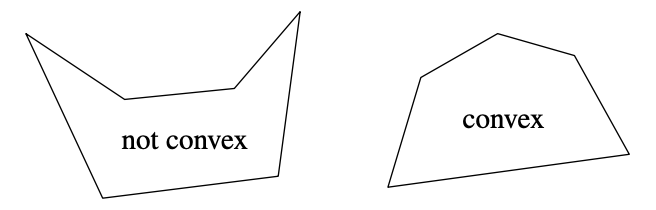
\includegraphics[scale=0.5]{images/bamo22-e3}            
        \end{center}
        Given a convex polygon, prove that one can find three distinct vertices $A$, $P$, and $Q$, where $PQ$ is a side of the polygon, such that the perpendicular from $A$ to the line $PQ$ meets the segment $PQ$ (possibly at $P$ or $Q$).
    % Answer: $\sqrt{2} + 1$
    \end{block}
\end{probslide}

\begin{probslide}[t]{CHMMC 2022, Individual \#5}{}
    \begin{block}{}
        Lin Lin has a $4\times4$ chessboard in which every square is initially empty. Every minute, she chooses a random square $C$ on the chessboard, and places a pawn in $C$ if it is empty. Then, regardless of whether $C$ was previously empty or not, she then immediately places pawns in all empty squares a king's move away from $C$.
        The expected number of minutes before the entire chessboard is occupied with pawns equals $\frac{m}{n}$ for relatively prime positive integers $m,n$. Find $m+n$.

        \textit{A king's move, in chess, is one square in any direction on the chessboard: horizontally, vertically, or diagonally.}
    % Answer: $28$
    \end{block}
\end{probslide}

\begin{probslide}[t]{HMMT February 2022, Guts \#18}{}
    \begin{block}{}
        Compute the number of permutations $\pi$ of the set $\{1, 2, \ldots , 10\}$ so that for all (not necessarily distinct) $m, n \in \{1, 2, \ldots , 10\}$ where $m + n$ is prime, $\pi(m) + \pi(n)$ is prime.
    % Answer: $4$
    \end{block}
\end{probslide}

\begin{probslide}[t]{PUMaC 2021, Division A, Combinatorics \#6}{}
    \begin{block}{}
        Alice, Bob, and Carol are playing a game. Each turn, one of them says one of the 3 players' names, chosen from {Alice, Bob, Carol} uniformly at random. Alice goes first, Bob goes second, Carol goes third, and they repeat in that order. Let $E$ be the expected number of names that are have been said when, for the first time, all 3 names have been said twice. If $E = \frac{m}{n}$ for relatively prime positive integers $m$ and $n$, find $m + n$. (Include the last name to be said twice in your count.)
    % Answer: $\sqrt{2} + 1$
    \end{block}
\end{probslide}

\begin{probslide}[t]{PUMaC 2021, Division A, Combinatorics \#7}{}
    \begin{block}{}
        Cassidy has string of $n$ bits, where $n$ is a positive integer, which initially are all 0s or 1s. Every second, Cassidy may choose to do one of two things:
        \begin{enumerate}
            \item Change the first bit (so the first bit changes from a 0 to a 1, or vice versa)
            \item Change the first bit after the first 1.
        \end{enumerate}
        Let $M$ be the minimum number of such moves it takes to get from $1 \ldots 1$ to $0 \ldots 0$ (both of length 12), and $N$ the number of starting sequences with 12 bits that Cassidy can turn into
        all 0s. Find $M + N$.
    % Answer: $\sqrt{2} + 1$
    \end{block}
\end{probslide}

\begin{probslide}[t]{BMT 2021, Geometry \#5}{}
    \begin{block}{}
        Let circles $\omega_1$ and $\omega_2$ intersect at $P$ and $Q$. Let the line externally tangent to both circles that is
        closer to $Q$ touch $\omega_1$ at $A$ and $\omega_2$ at $B$. Let point $T$ lie on segment $\overline{PQ}$ such that $\angle{ATB} = 90^\circ$.
        Given that $AT = 6, BT = 8,$ and $P T = 4$, compute $P Q$.
    % Answer: $\frac{56}{9}$
    \end{block}
\end{probslide}


\end{document}
